\documentclass{article}
\usepackage{amsmath}
\usepackage{hyperref}
\usepackage{float}
\usepackage{graphicx}
\usepackage{caption}

\author{Erin Angelini}
\title{*Updated* Documentation for \texttt{C++} model}
\begin{document}
\maketitle
\section{Updates to \texttt{main.cpp}:}
The main file now includes code that writes the end time and angular orientation of the spindle when it has completed rotation. The first part of this code is the part that determines what ``complete'' rotation means. Experimental results from the Dawes lab indicate that nuclear envelope breakdown occurs within 90\% of the full rotation from $\pi/2$ to the horizontal. Therefore, under the \texttt{runModel} function, we place a check on the spindle's angle to see if it is within $\pi/2 \pm 0.9(\pi/2)$. If it has reached this threshold, we consider to be done rotating, so we write the final time and position and end the run.

The new function that writes the final time for us is called \texttt{writeFinalTime}; its writes the final spindle position, angle, and time to rotation. As of right now, this feature(i.e. recording time to rotate) is turned on and off manually by respectively uncommenting and commenting out these two blocks of code. These blocks of code can be found by searching the document for the comment string \texttt{//EA:}.

\subsection{Length dependence}
There is also a version of \texttt{main.cpp} that includes length dependent pulling and pushing forces. This change is implemented under the functions \texttt{mtForceCalcM} and \texttt{mtForceCalcD}, which are the functions that calculate the total force generated by the mother (M) and daughter (D) asters, respectively. As with the current implementation of the mean-field model, each MT force scales with its length \texttt{L} by a factor of $\beta = 1$. That is, force(MT$_i$) = L$_i$ for each MT. Like the other updates, this code is marked by the comment \texttt{//EA:} and must be turned on and off manually.

\section{Updates to \texttt{parameters.cpp}:}
For the off-center spindle position option (i.e. \texttt{startPsi} $> 0$), the off-center coordinate is no longer fixed at 10.0 but instead scales with \texttt{R1\_max}. More specifically it is set to be 0.4$\times$\texttt{R1\_max}, which is the 70:30 egg-length point (consistent with the results form Coffman \emph{et al.}).

The \texttt{parameters.cpp} file also now includes code for implementing a lower anterior MT-dynein binding probability ($P_a = 0.65$, coded into \texttt{regionForceMultipliers}) \emph{without} push bands present. In this implementation, the anterior and posterior regions are defined by the parameter \texttt{myPos}, which is the Cartesian angle that marks the 60:40 egg-length point (0.2$\times$\texttt{R1\_max}). This parameter is used to divide the cortex into 3 regions: (upper) posterior, anterior, and (lower) posterior. Like the new code in \texttt{main.cpp}, turning these features `on' or `off' must be done manually by uncommenting/commenting out the appropriate code.

\begin{figure}[H]
\centering
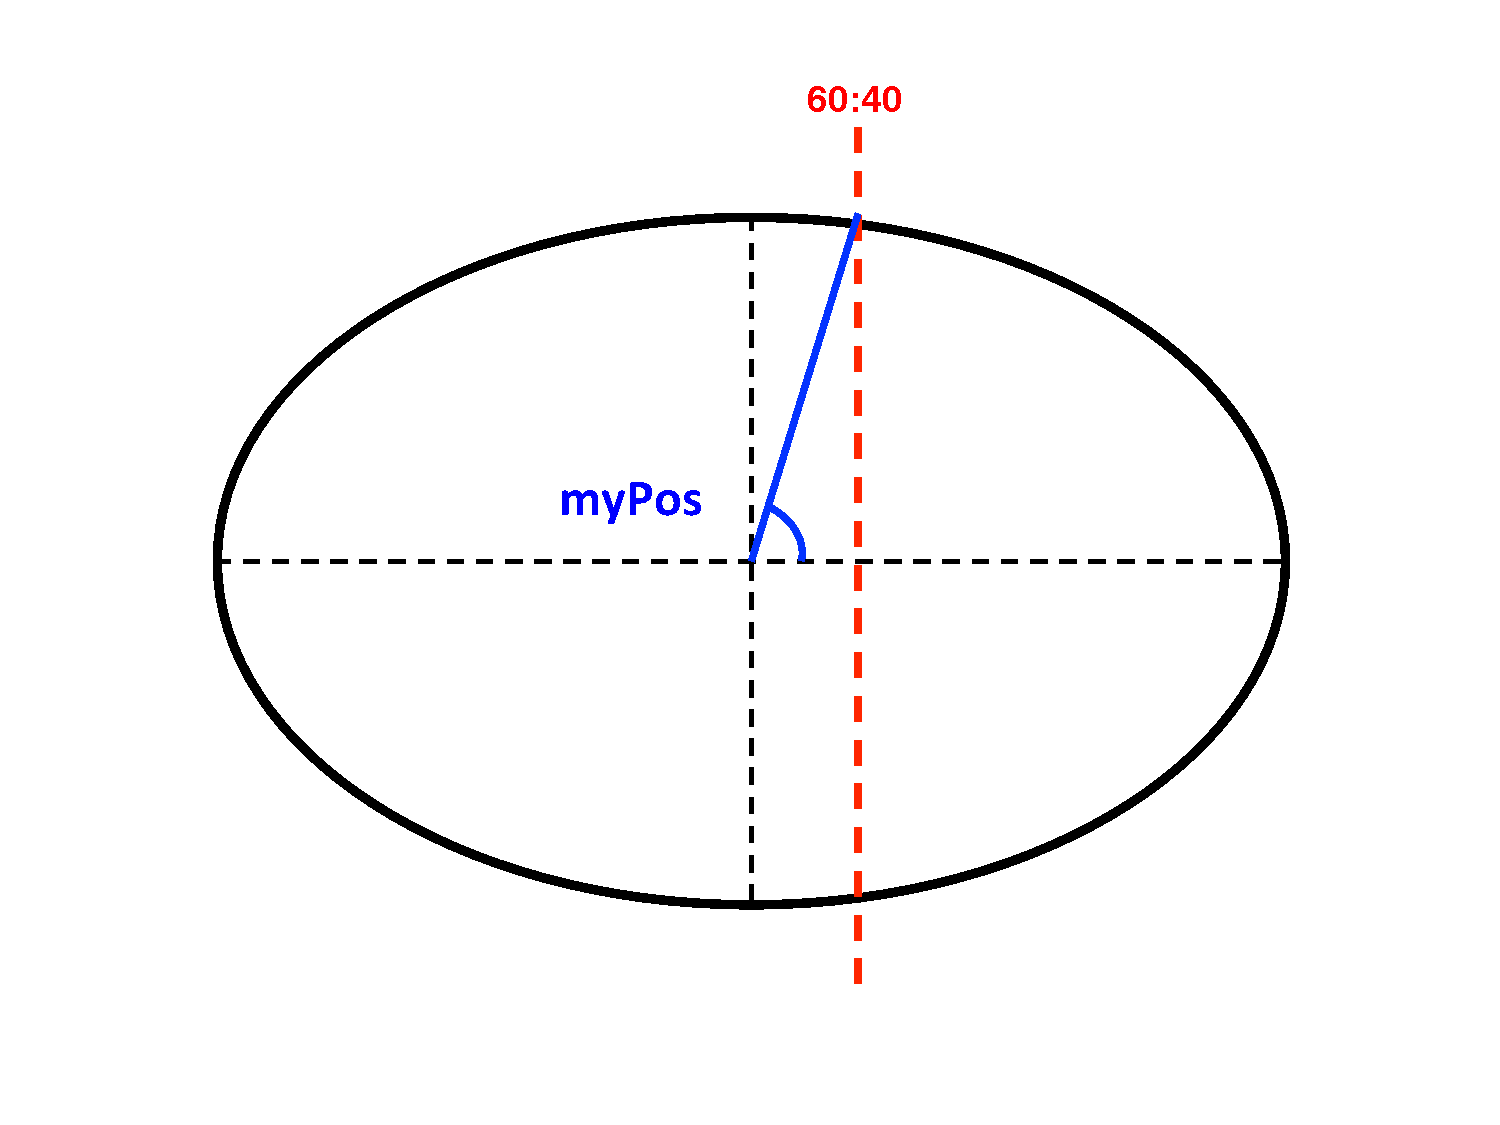
\includegraphics[width=0.9\textwidth]{figures/APsetup.pdf}
\caption{Demarcation of the 60:40 anterior-to-posterior split by Cartesian angle in the computational model.}
\label{divplane}
\end{figure}

\subsection{Changing parameters with aspect ratio}
Certain parameters need to be updated when you change the value of either \texttt{R1\_max} or \texttt{R2\_max} (i.e. the length of either axis of the ellipse). The instructions for doing so are as follows. So far all changes must be done manually (i.e. copy and paste for each new aspect ratio)
\begin{description}
  \item[\texttt{myPos}:] The position of the anterior-to-posterior break. If implementing the model with an anterior-to-posterior difference in binding probabilities without a push band, then this parameter must be updated with the aspect ratio. The pre-calculated values are located under the `band and window code' directory in the file \texttt{APpos.cpp}.
  \item[\texttt{start} and \texttt{end}:] These are the Cartesian angles the demarcate the start and the end of the push band regions, respectively. If implementing the model with the push bands, these parameters also change with aspect ratio. The pre-calculated values are located under the `band and window code' directory in the file \texttt{pushBands.cpp}.
  \item[\texttt{numberContactWindows} and \texttt{contactWindowAngles}] These inputs describe the number of cortical dyneins and their positions (in \emph{polar} angles, NOT Cartesian), respectively. These must also be updated with aspect ratio. The pre-calculated values are located under the `band and window code' directory in the file \texttt{aspectContactWindows.cpp}.
\end{description}

\section{General use}
This code requires Xcode to run on Mac computers. To run the model, first open terminal and cd into the folder containing \texttt{main.cpp} and the other model files (\texttt{parameters.cpp}, \texttt{mtKineticModel.exe}, etc.). On the command line, enter \texttt{`make'} \textendash this command compiles the model. Then enter \texttt{`./mtKineticModel n fileName'}, where \texttt{n} is the desired number of runs and \texttt{fileName} is the name of the .csv file to which the final data will be written. To read more about the options for writing final data, see the `README\_2016' file (original documentation written by Matt McDermott). If no options are passed into the command line about what data is written into the .csv file, then the program automatically writes the final position of the pronucleus ($x$ and $y$ coordinates) and the final angular orientation of the spindle (radians). If the \texttt{writeFinalTime} function is in place, then the program also writes the time at which the spindle completed rotation (in minutes). If the spindle does not complete rotation, no time is written and the final time is the total length of the simulation (as given in the \texttt{parameters.cpp} file). The .csv file and question is written to the folder titled `data,' which is located one directory up from the model code itself.

\end{document}
